\subsection{Architecture}

We have designed the server by the layered approach of MVC (figure
\ref{fig:server_architecture}).

\begin{figure}[h]
	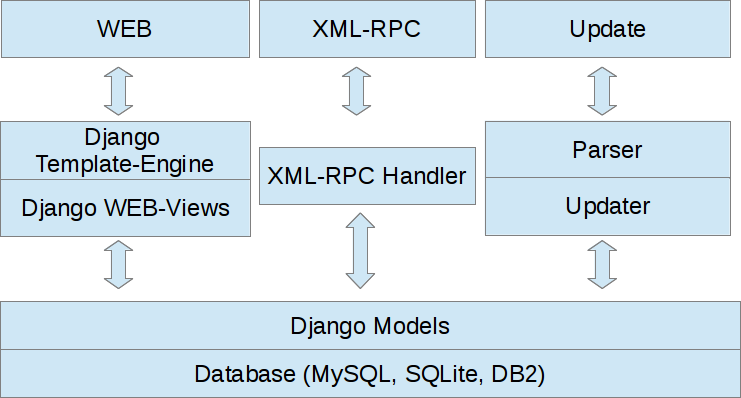
\includegraphics[width=130mm]{./img/Server-MVC.png}
	\caption{Server Architecture}
	\label{fig:server_architecture}
\end{figure}

The web-interface uses pure \django{} logic. The HTML visible in the users
browser is generated by the \django{} template-engine, which recieves its data
from the views created by using ordinary Python code.

The XML-RPC server uses a handler which is administering the connections to
and from the sensors, and exposing the relevant methods to allow the sensors to
do a synchronization.

The update module is used for unpacking and preparing the update files for
parsing. It then handles the files to the parser. This parser is then tasked
with translating the raw rule files into more managable datastructures for the
Updater, which in turn saves them to the database.

Finally, common for all the interfaces is the \django{} Models. We use the
database abstraction layer provided by \django{} to map the rows of a
relational database into \django{} objects. This is the part that lets us write
code which is compatable with several different database engines.